\documentclass[11pt, a4paper]{article}
\usepackage{pdfpages}
\usepackage{parallel}
\usepackage[T2A]{fontenc}
%\usepackage{ucs}
\usepackage[utf8]{inputenc}
\usepackage[english,russian]{babel}
\usepackage{hyperref}
\usepackage{rotating}
\usepackage[inner=2cm,top=1.8cm,outer=2cm,bottom=2.3cm,nohead]{geometry}
%\usepackage{listings}
\usepackage{graphicx}
\usepackage{wrapfig}
\usepackage{longtable}
\usepackage{indentfirst}
\usepackage{array}
\usepackage{tikzsymbols}
\usepackage{soul}
\usepackage[ruled,vlined]{algorithm2e}
\usepackage{qrcode}
\counterwithout{figure}{section} 

\usepackage{url}
\makeatletter
\g@addto@macro{\UrlBreaks}{\UrlOrds}
\makeatother

\newcolumntype{P}[1]{>{\raggedright\arraybackslash}p{#1}}
\frenchspacing
%\usepackage{fixltx2e} %text sub- and superscripts
\usepackage{icomma} % коскі ў матэматычным рэжыме
%\PreloadUnicodePage{4}

\newcommand{\longpage}{\enlargethispage{\baselineskip}}
\newcommand{\shortpage}{\enlargethispage{-\baselineskip}}

\def\switchlang#1{\expandafter\csname switchlang#1\endcsname}
\def\switchlangbe{
\let\saverefname=\refname%
\def\refname{Літаратура}%
\def\figurename{Іл.}%
}
\def\switchlangru{
\let\saverefname=\refname%
\let\savefigurename=\figurename%
\def\refname{Литература}%
\def\figurename{Рис.}%
}
\def\switchlangen{
\let\saverefname=\refname%
\def\refname{References}%
\def\figurename{Fig.}%
}

\hyphenation{admi-ni-stra-tive}
\hyphenation{ex-pe-ri-ence}
\hyphenation{fle-xi-bi-li-ty}
\hyphenation{Py-thon}
\hyphenation{ma-the-ma-ti-cal}
\hyphenation{re-ported}
\hyphenation{imp-le-menta-tions}
\hyphenation{pro-vides}
\hyphenation{en-gi-neering}
\hyphenation{com-pa-ti-bi-li-ty}
\hyphenation{im-pos-sible}
\hyphenation{desk-top}
\hyphenation{elec-tro-nic}
\hyphenation{com-pa-ny}
\hyphenation{de-ve-lop-ment}
\hyphenation{de-ve-loping}
\hyphenation{de-ve-lop}
\hyphenation{da-ta-ba-se}
\hyphenation{plat-forms}
\hyphenation{or-ga-ni-za-tion}
\hyphenation{pro-gramming}
\hyphenation{in-stru-ments}
\hyphenation{Li-nux}
\hyphenation{sour-ce}
\hyphenation{en-vi-ron-ment}
\hyphenation{Te-le-pathy}
\hyphenation{Li-nux-ov-ka}
\hyphenation{Open-BSD}
\hyphenation{Free-BSD}
\hyphenation{men-ti-on-ed}
\hyphenation{app-li-ca-tion}

\def\progref!#1!{\texttt{#1}}
\renewcommand{\arraystretch}{2} %Іначай формулы ў матрыцы зліпаюцца з лініямі
\usepackage{array}

\def\interview #1 (#2), #3, #4, #5\par{

\section[#1, #3, #4]{#1 -- #3, #4}
\def\qname{LVEE}
\def\aname{#1}
\def\q ##1\par{{\noindent \bf \qname: ##1 }\par}
\def\a{{\noindent \bf \aname: } \def\qname{L}\def\aname{#2}}
}

\def\interview* #1 (#2), #3, #4, #5\par{

\section*{#1\\{\small\rm #3, #4. #5}}
\ifx\ParallelWhichBox\undefined%
    \addcontentsline{toc}{section}{#1, #3, #4}%
\else%
\ifnum\ParallelWhichBox=0%
    \addcontentsline{toc}{section}{#1, #3, #4}%
\fi\fi%

\def\qname{LVEE}
\def\aname{#1}
\def\q ##1\par{{\noindent \bf \qname: ##1 }\par}
\def\a{{\noindent \bf \aname: } \def\qname{L}\def\aname{#2}}
}

\newcommand{\interviewfooter}[1]{
\vskip 1em
\noindent \textit{#1}
}

\AtEndDocument{\vfill\centering \qrcode{https://github.com/fiowro/mouses/blob/main/\jobname.pdf}}

\switchlang{ru}
\begin{document}

\title{1986 "--- Sunnyline DIGIMOUSE}
\date{}
\maketitle
\selectlanguage{russian}

Мышь Sunnyline Digimouse для IBM-совместимых компьютеров с последовательным интерфейсом очевидно является первой мышью, выпущенной под брэндом Sunnyline.
Мыши под этим брэндом продавались компанией Sunnyline MultiMedia Products AG в Германии в конце 80-х и в 90-е годы. Sunnyline не имела собственного производства и размещала заказы в других компаниях на контрактной основе. В частности, создателем данной мыши была компания Dubois Depraz SA "--- известный швейцарский производитель часов, занимавшийся производством оптомеханических мышей в 1980-х годах на основе дизайна, разработанного Жаном-Даниэлем Нику и Андре Гиньяром в Федеральной политехнической школе Лозанны.

После выпуска мышей P4 и P1000 под собственным брэндом совместно с никому неизвестной на тот момент Logitech, Depraz полностью переключилась на контрактную разработку для других компаний, активно предоставляя собственные мыши для ребрендинга и разрабатывая их на заказ на базе своих типовых конструкций. Наиболее активным заказчиком мышей Depraz выступала британская компания Advanced Memory Systems (AMX): плодами этого сотрудничества стали несколько моделей мышей, продававшихся под одним и тем же названием <<AMX Mouse>>.

Как можно заметить, для своей первой мыши Sunnyline заказала Depraz разработку нестандартного дизайна корпуса, характерный именно для данной модели (рис. \ref{fig:SunnylineDIGIMOUSEPic}) и не появлявшийся в мышах других компаний.

\begin{figure}[h]
   \centering
    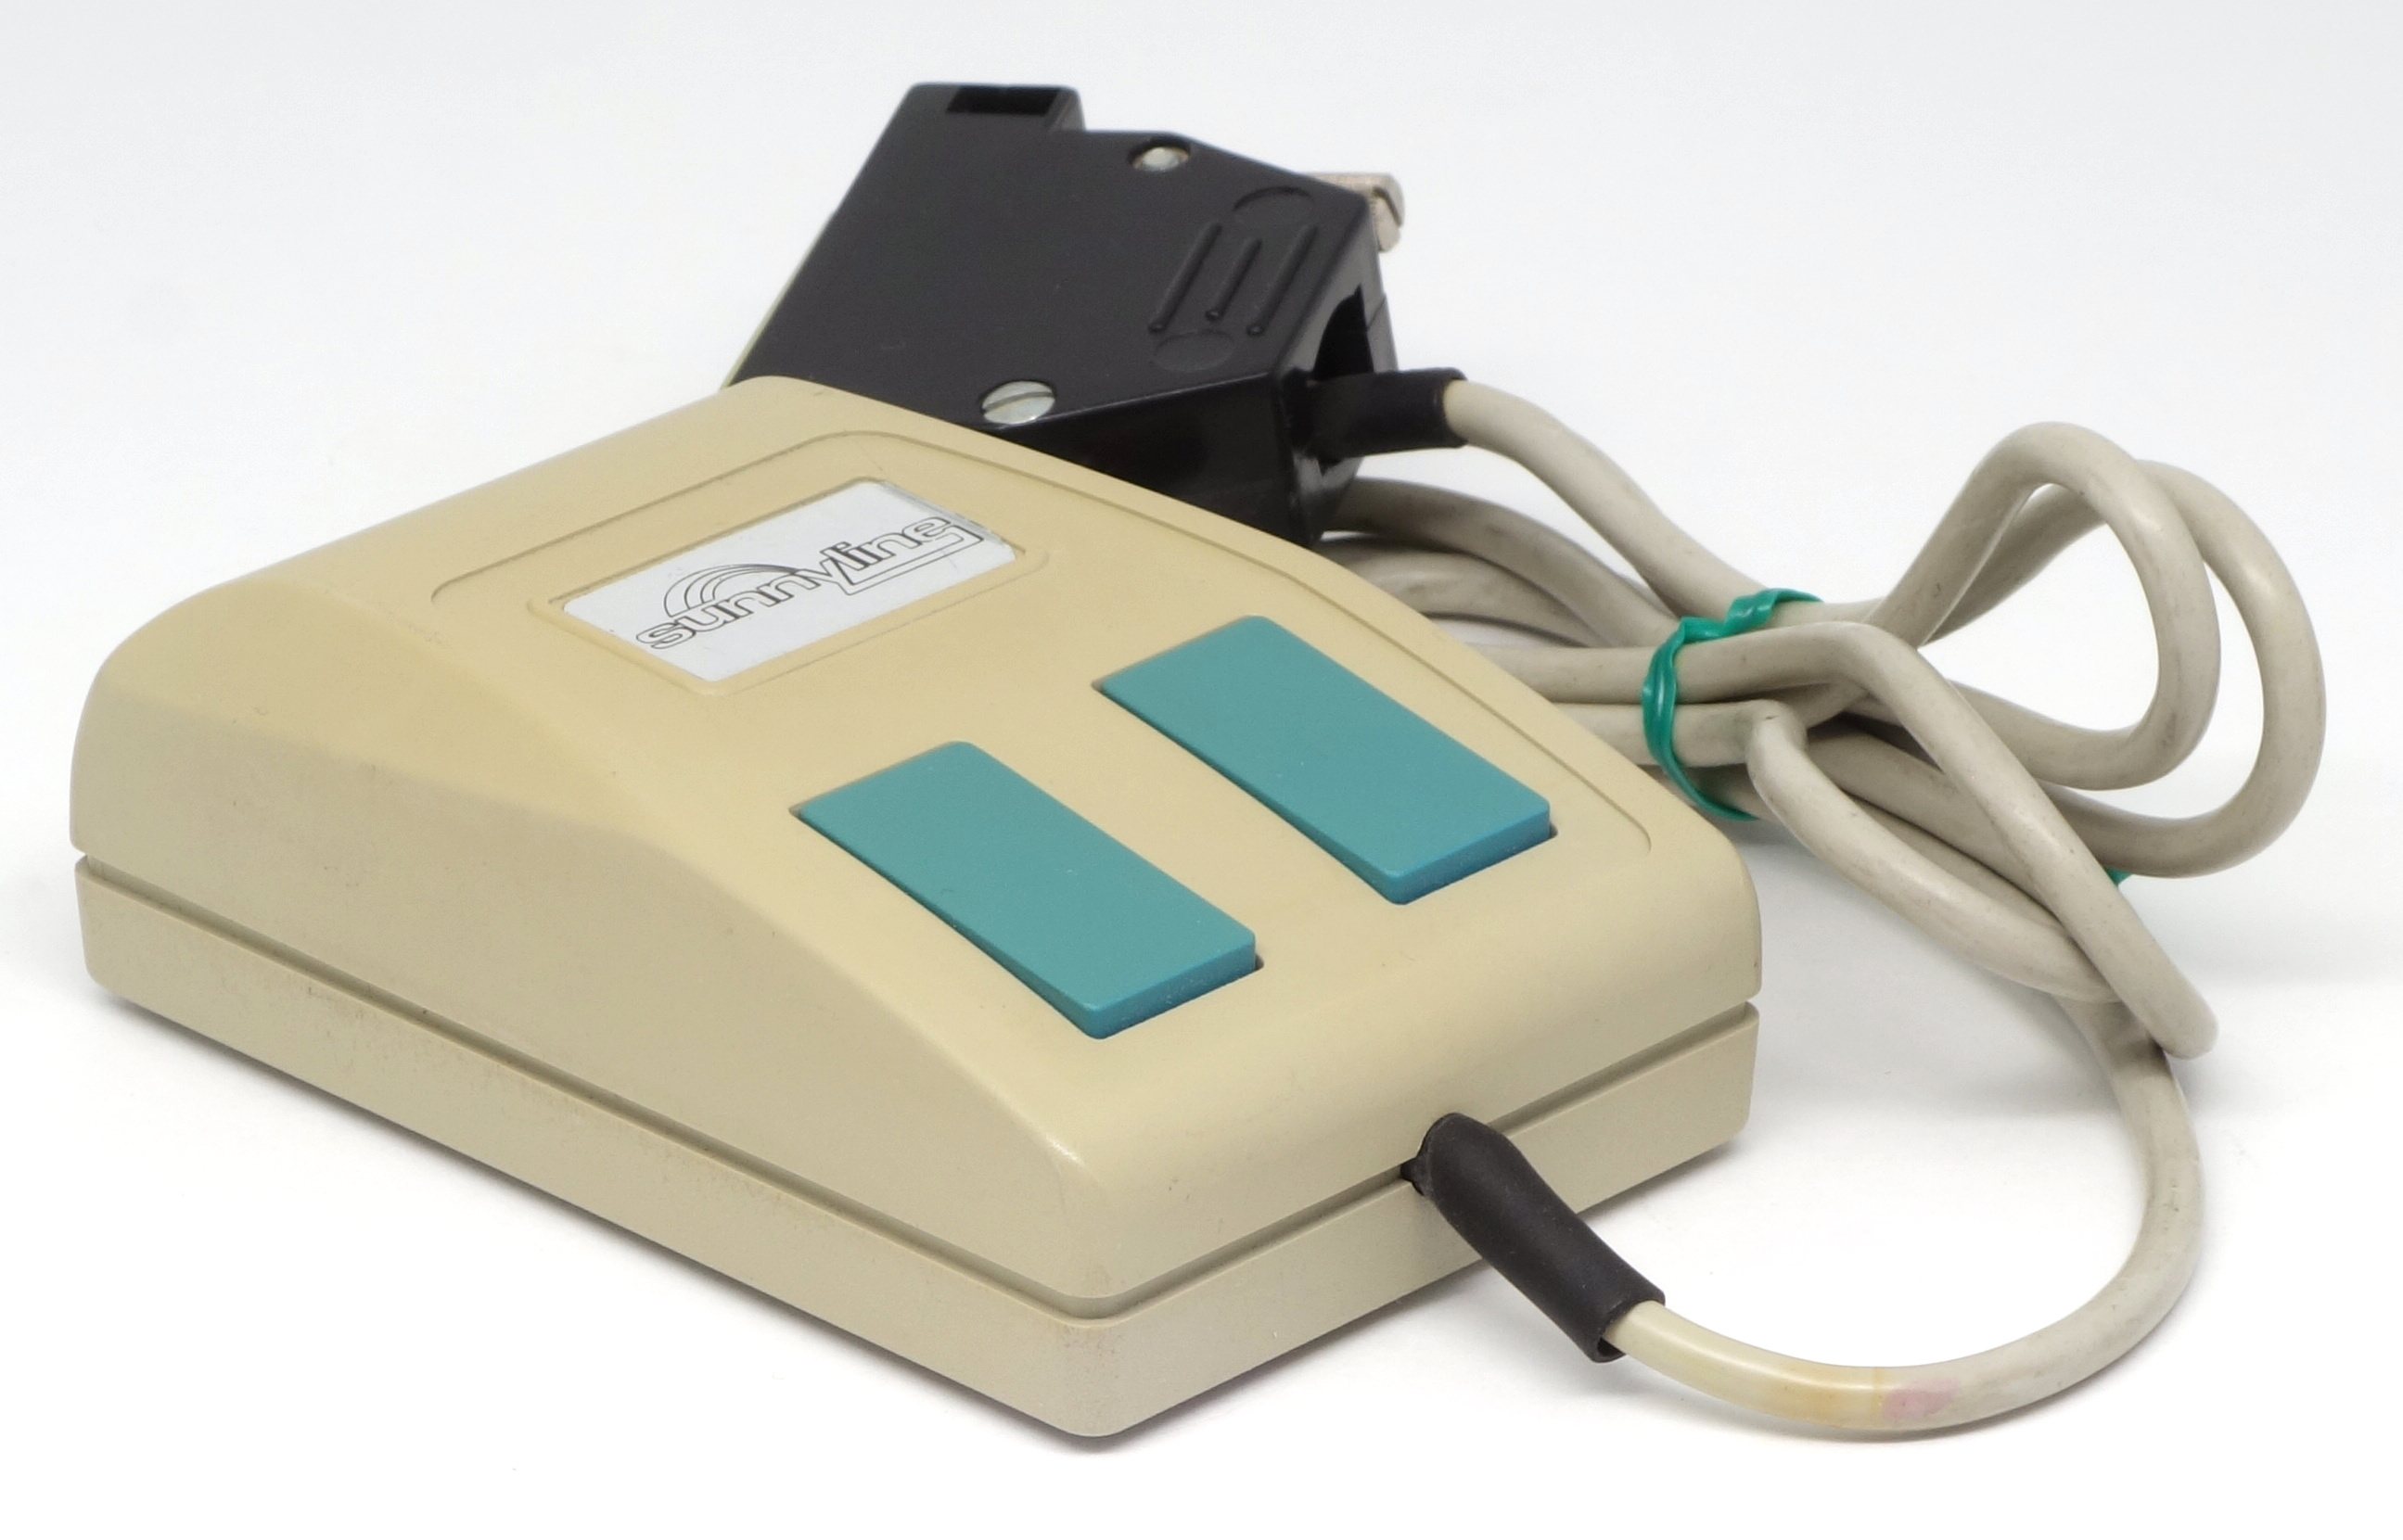
\includegraphics[scale=0.75]{1986_sunnyline_digimouse/pic_30.jpg}
    \caption{DIGIMOUSE}
    \label{fig:SunnylineDIGIMOUSEPic}
\end{figure}

В результате мышь получила уникальную верхнюю часть корпуса, в то время как нижняя часть (рис. \ref{fig:SunnylineDIGIMOUSETopAndBottom}) практически идентична мыши AMX mouse 2 поколения, выпущенной Depraz в том же самом 1986 году.
Низ обеих моделей демонстрирует ряд элементов, изначально появившихся в мыши Depraz Digimouse P1000: шар из полимерного материала, закрепленное шурупом съемное кольцо для чистки мыши, а также ограничитель, защищающий выход кабеля из корпуса мыши от повреждений. Наклейка на нижней стороне мыши Sunnyline содержит информацию о швейцарском происхождении мыши, а также название модели <<DIGIMOUSE D 86 S>>. Хотя какие-либо обзорные или рекламные публикации о данной модели неизвестны, предположение, что в номере содержится год выпуска, а также то, что компания Sunnyline MultiMedia Products AG была основана именно в 1986 году \cite{Sunnyline}, позволяют считать данную модель первой мышью Sunnyline.

\begin{figure}[h]
    \centering
    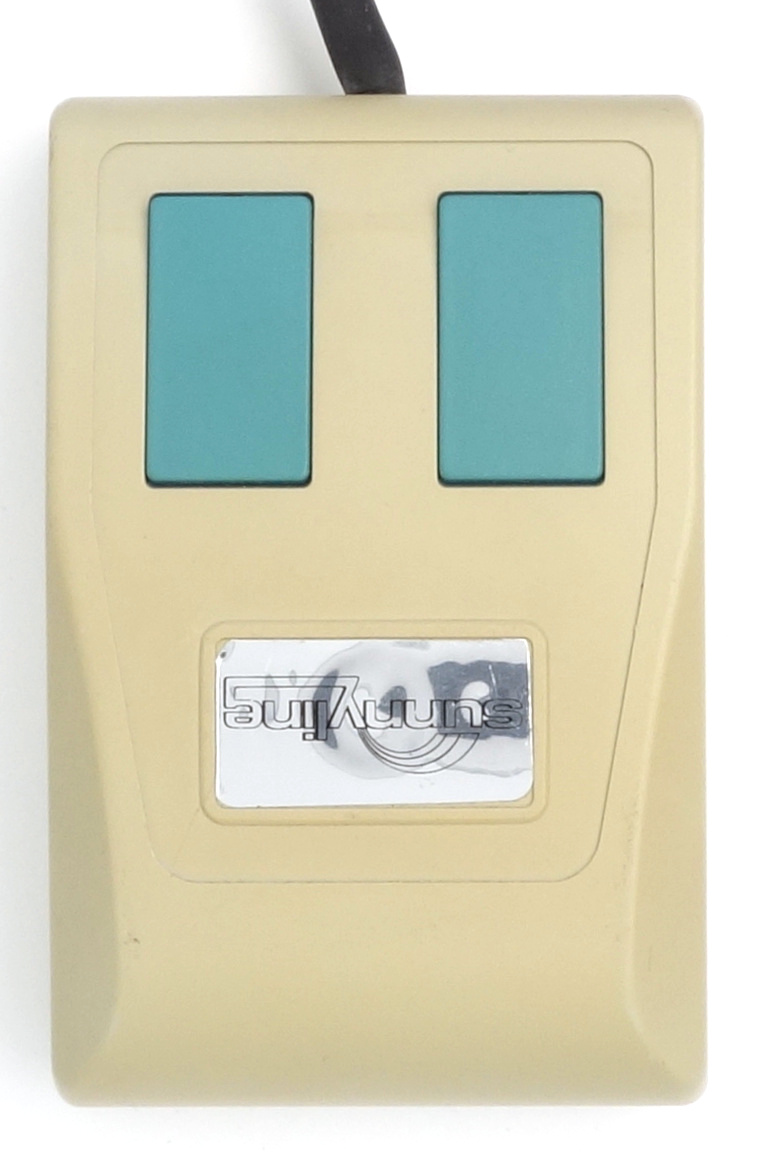
\includegraphics[scale=0.8]{1986_sunnyline_digimouse/top_30.jpg}
    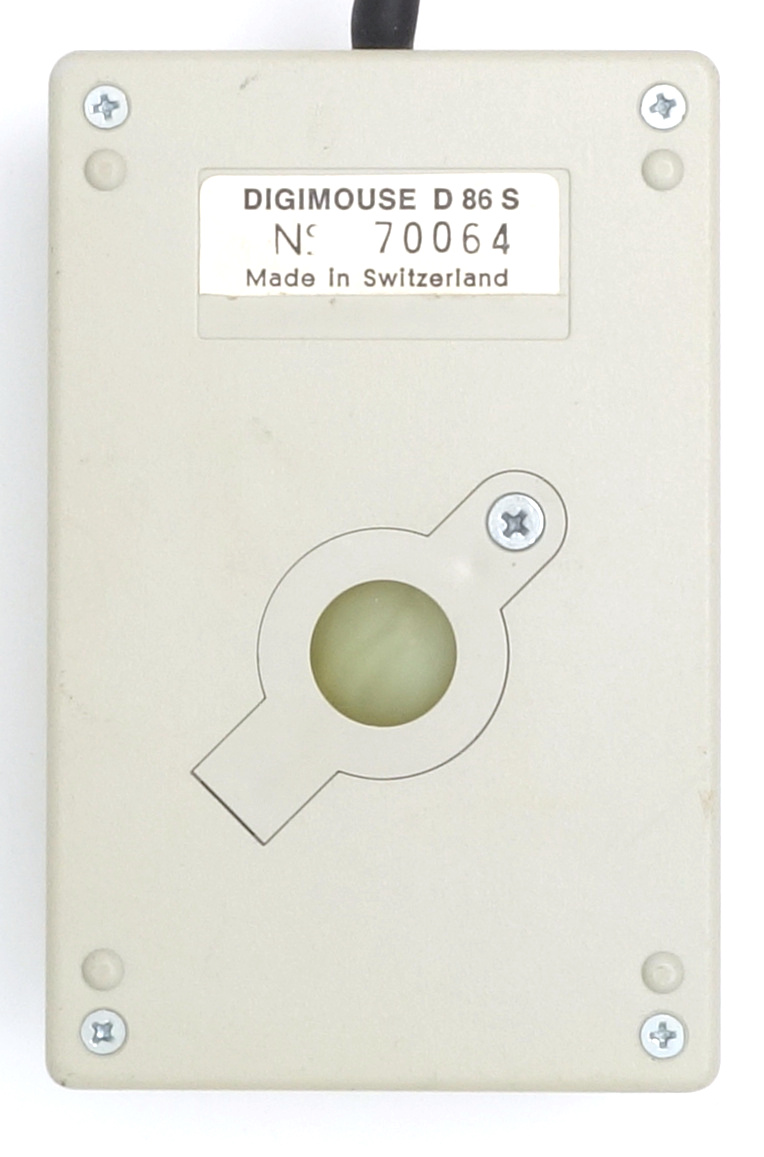
\includegraphics[scale=0.8]{1986_sunnyline_digimouse/bottom_30.jpg}
    \caption{DIGIMOUSE, вид сверху и снизу}
    \label{fig:SunnylineDIGIMOUSETopAndBottom}
\end{figure}

В отличие от своего близкого родственника "--- мыши AMX для компьютеров BBC Micro "--- Sunnyline DIGIMOUSE имеет две а не три кнопки (рис. \ref{fig:SunnylineDIGIMOUSETopAndBottom}) и бежевый корпус, который вписывается в габариты мыши AMX, но усовершенствован скошенными гранями и закруглением в зоне запястья. На верхней стороне присутствует металлическая накладка с эмблемой Sunnyline, а также контрастные зелёные кнопки. Очевидно, кнопки апеллируют к цветовой схеме первой мыши Microsoft, выпущенной тремя годами ранее и известной как <<Зеленоглазая мышь>>, поэтому технически Sunnyline DIGIMOUSE могла бы получить известность под названием <<зеленоглазая мышь Sunnyline>>, будь она выпущена в более заметных количествах.
В последующих моделях Sunnyline следовала по более экономному пути, используя готовые дизайны корпусов компаний-производителей без существенных модификаций.

\begin{figure}[h]
    \centering
    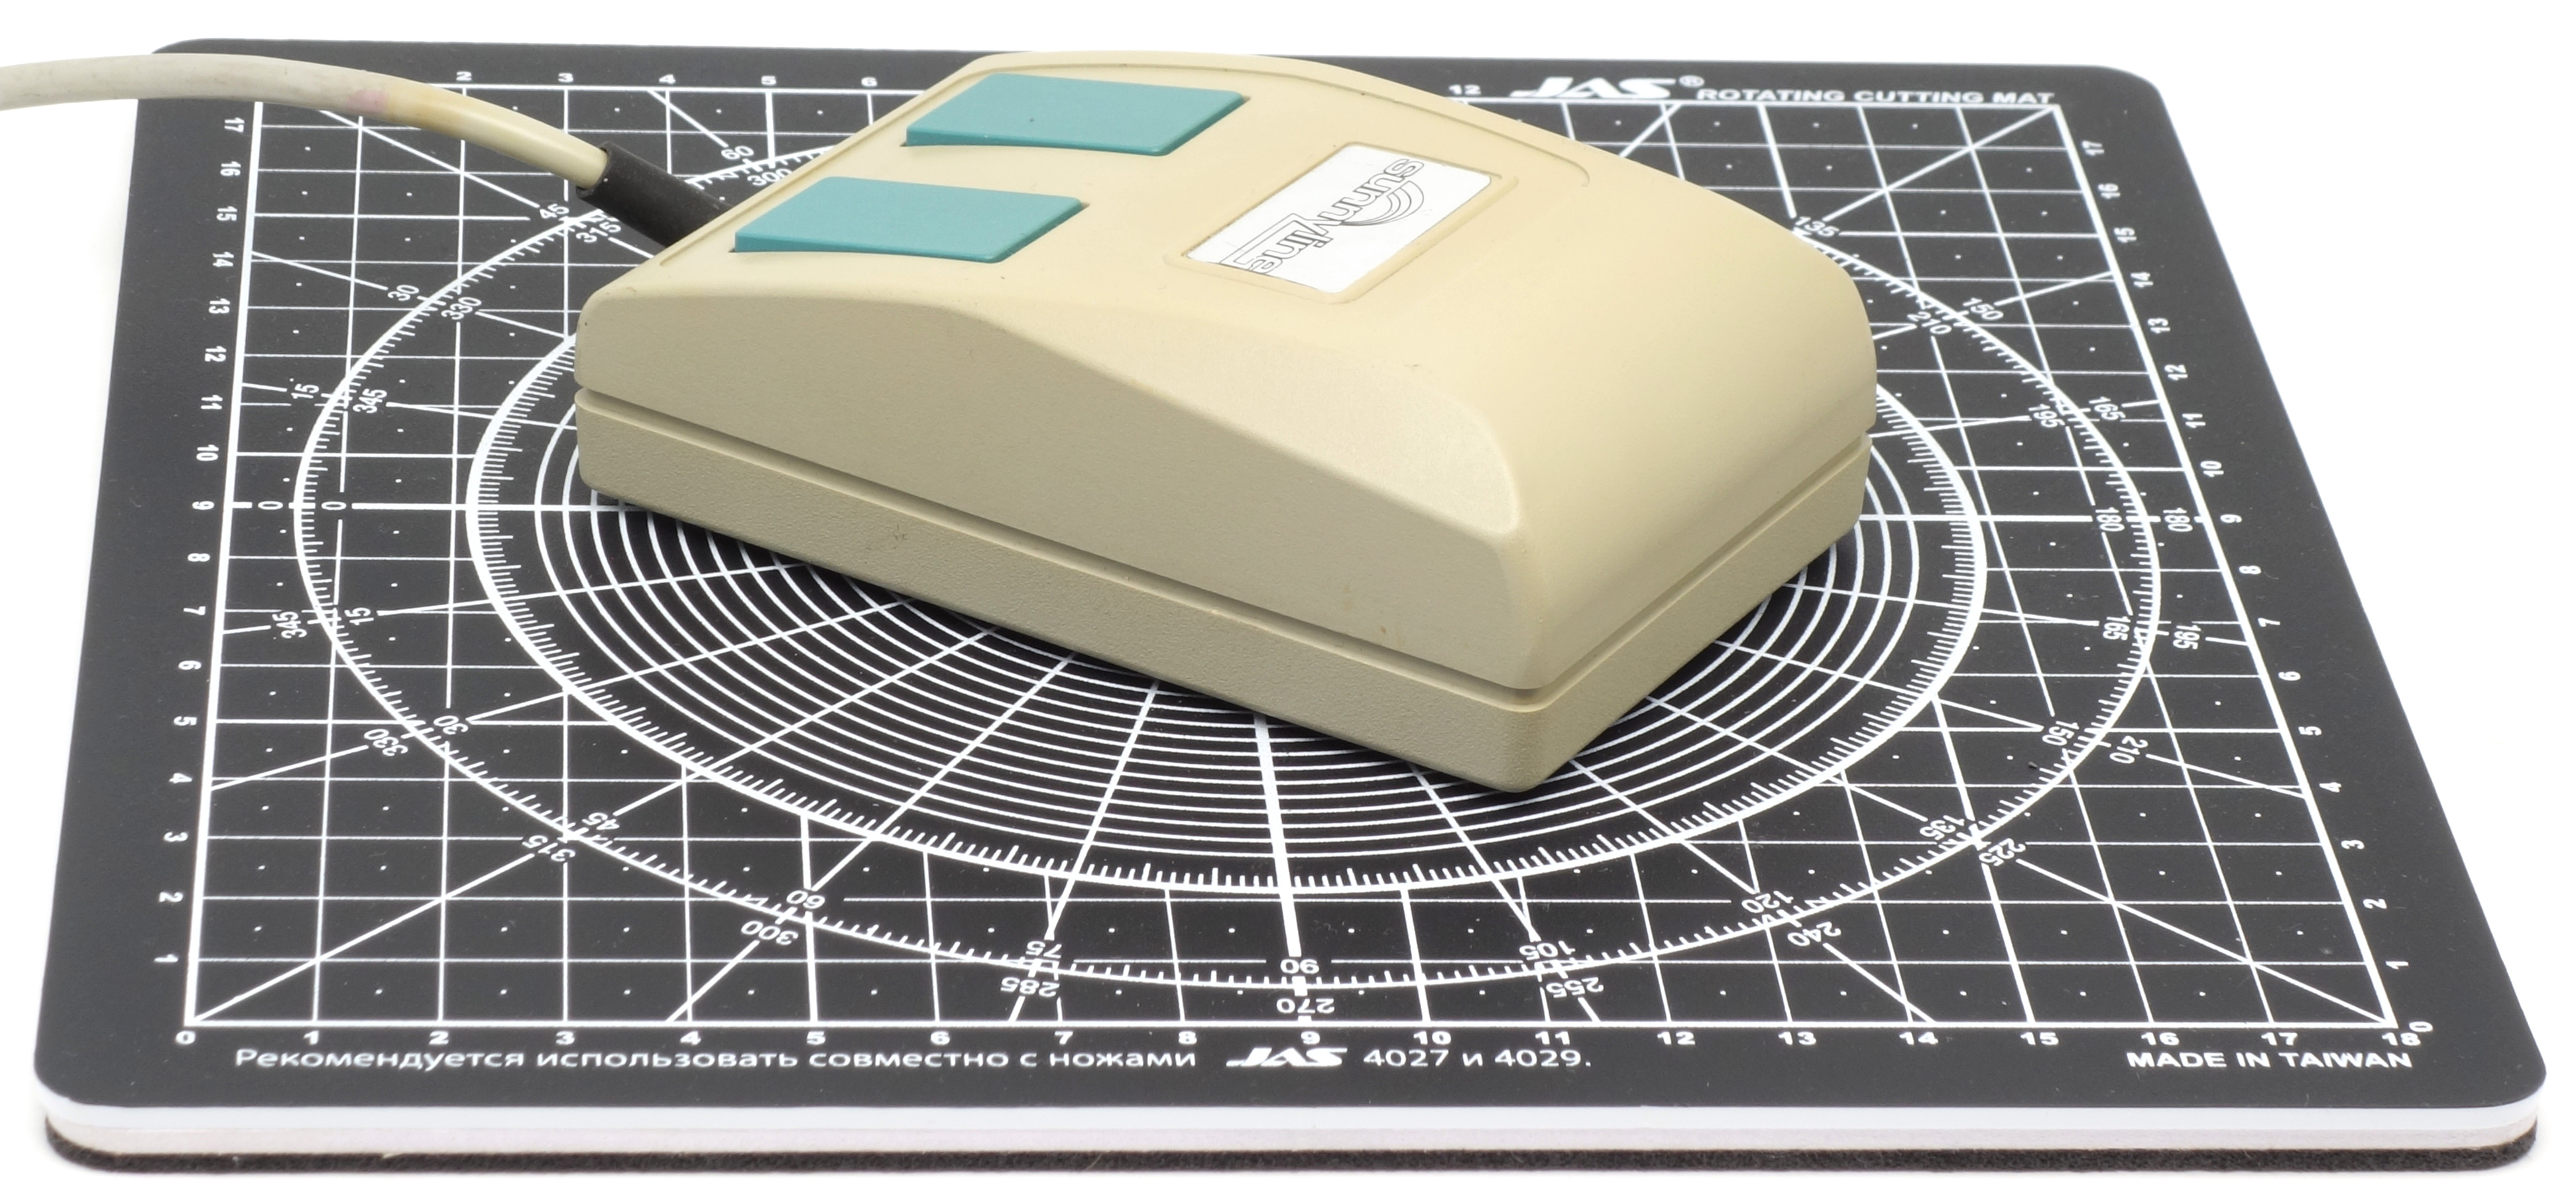
\includegraphics[scale=0.55]{1986_sunnyline_digimouse/size_30.jpg}
    \caption{DIGIMOUSE на размерном коврике с шагом сетки 1~см}
    \label{fig:SunnylineDIGIMOUSESize}
\end{figure}

Мышь имеет размеры, типичные для мышей 1980-х годов (рис. \ref{fig:SunnylineDIGIMOUSESize}).

\begin{figure}[h]
    \centering
    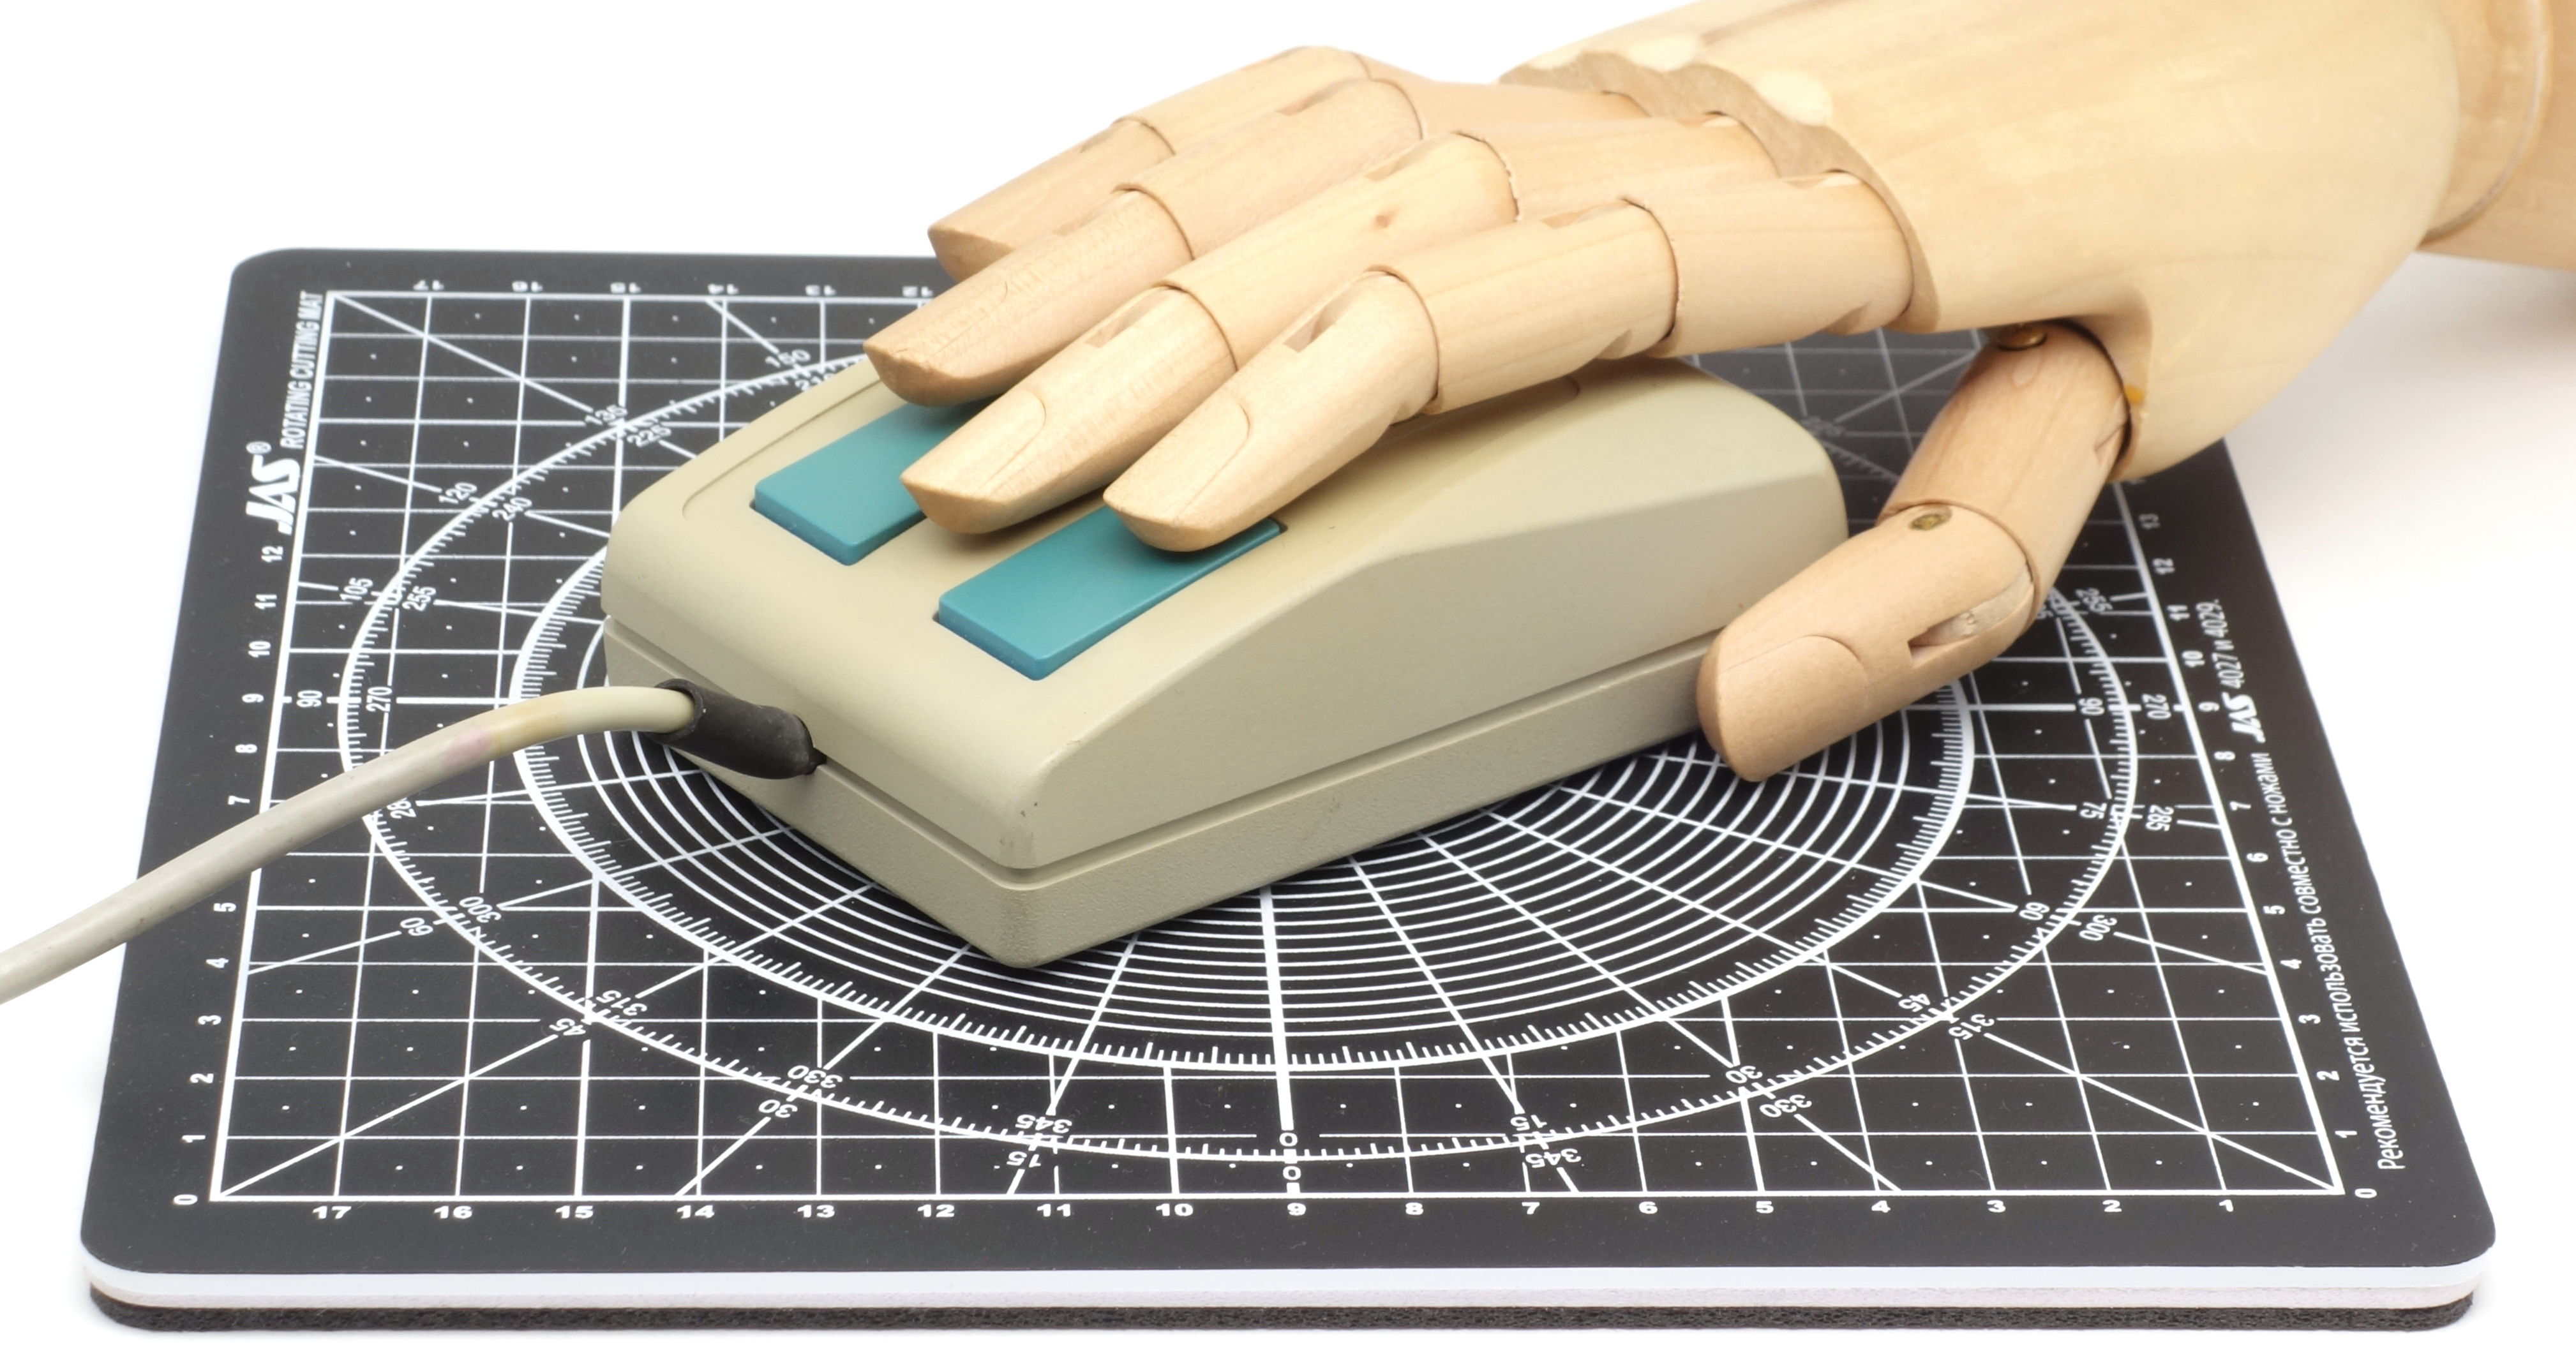
\includegraphics[scale=0.55]{1986_sunnyline_digimouse/hand_30.jpg}
    \caption{DIGIMOUSE с моделью руки человека}
    \label{fig:SunnylineDIGIMOUSEHand}
\end{figure}

Кнопки Sunnyline DIGIMOUSE имеют достаточно большую площадь, что обеспечивает их вполне комфортное нажатие пальцами. В целом, закругленные ребра корпуса оказывают некоторое положительное влияние на эргономику, однако типичная для мышей 80-х годов форма не предоставляет существенной опоры для ладони (рис. \ref{fig:SunnylineDIGIMOUSEHand}).

\begin{figure}[h]
    \centering
    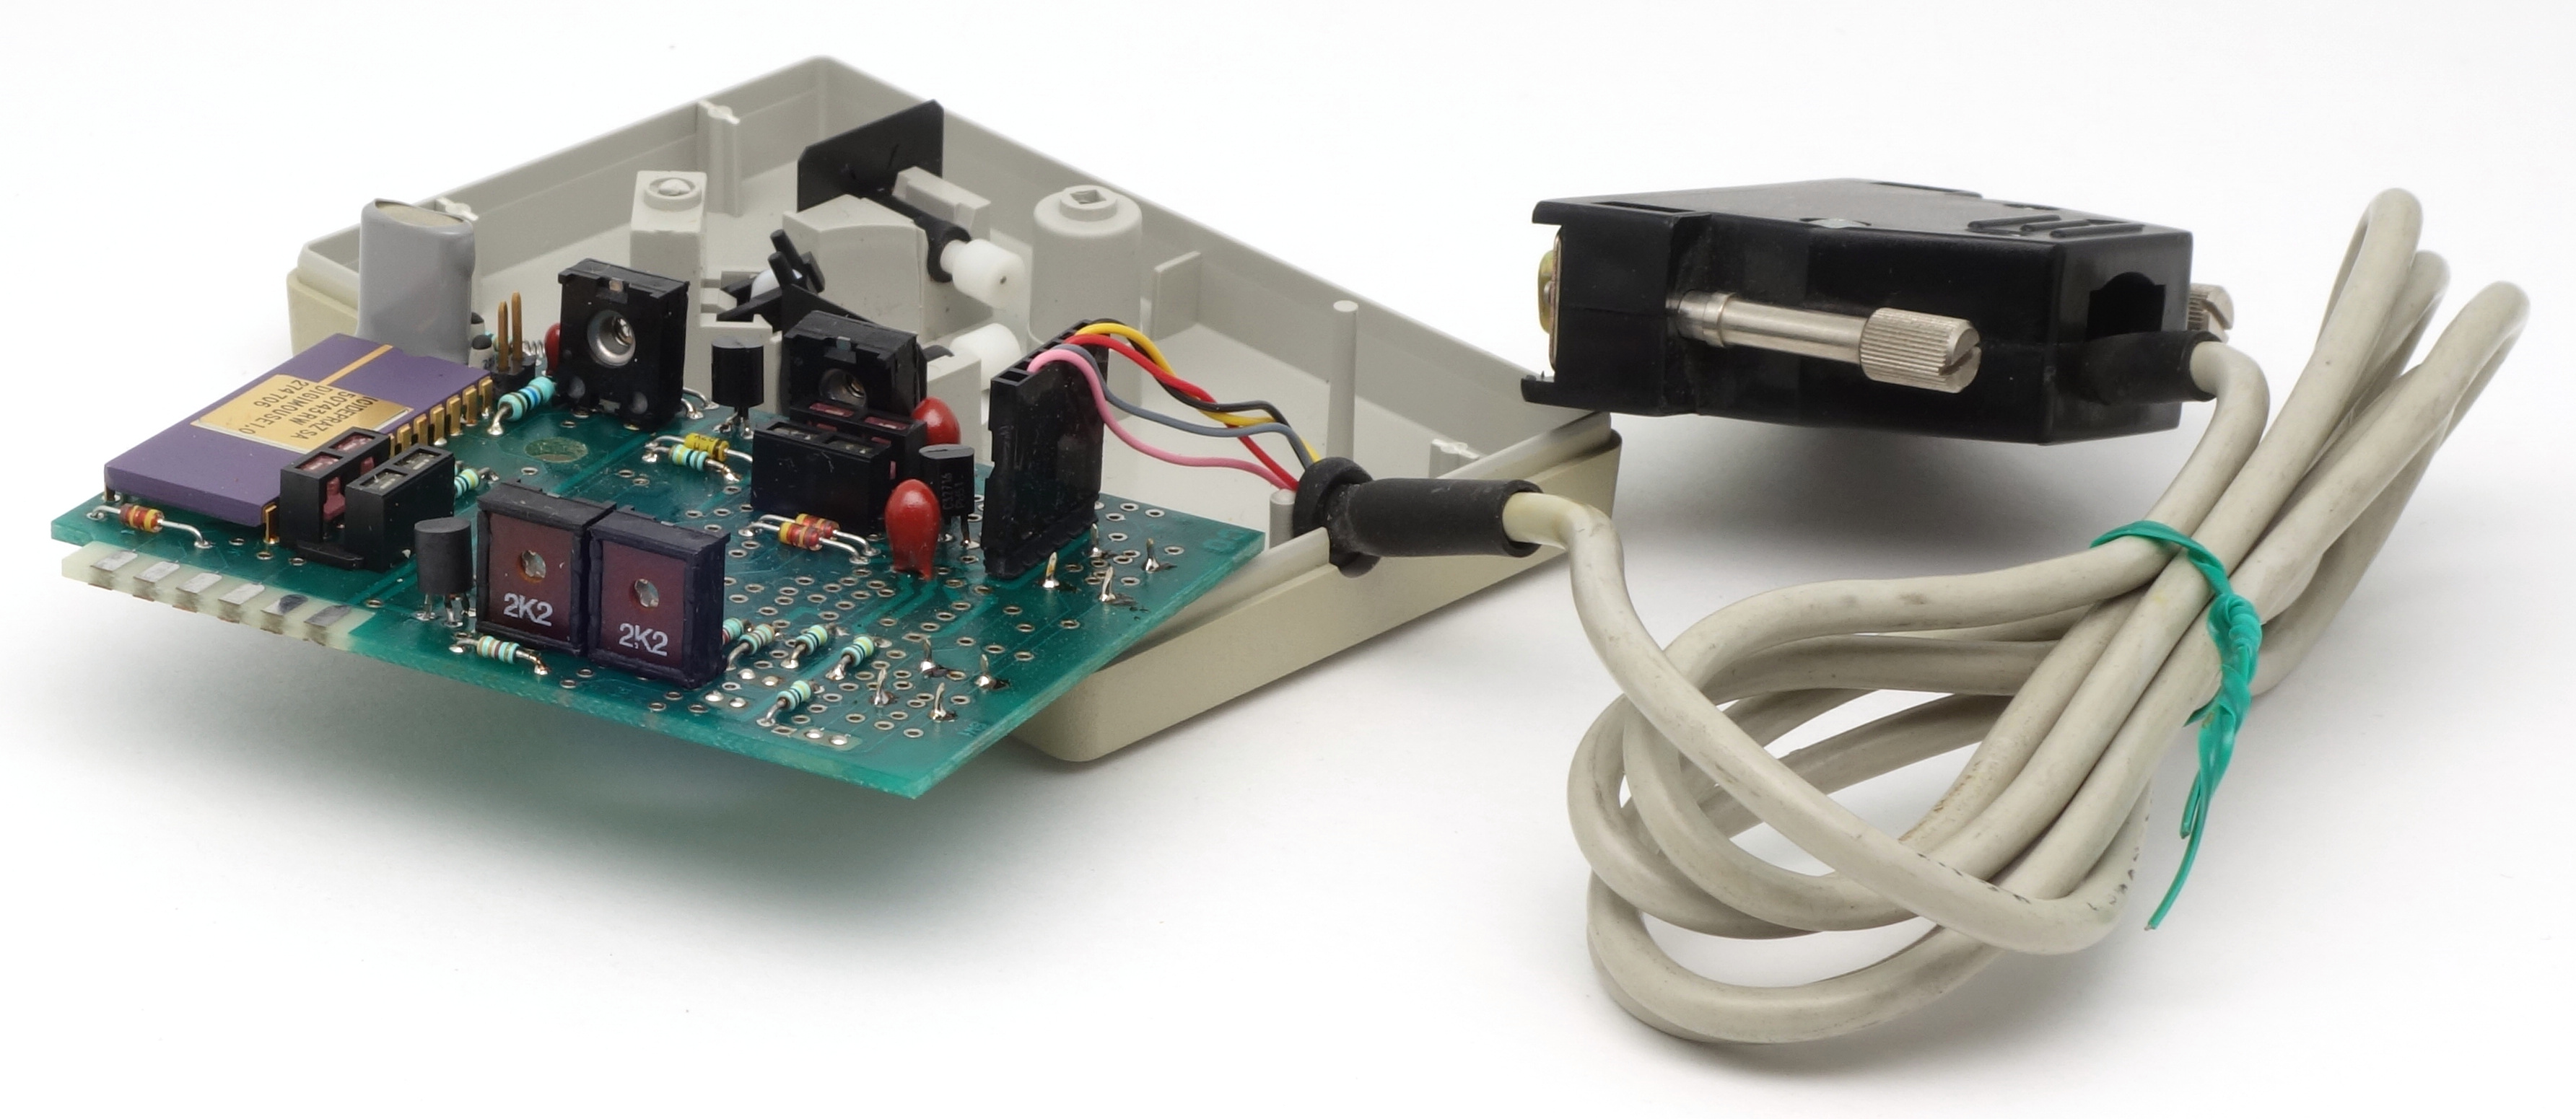
\includegraphics[scale=0.65]{1986_sunnyline_digimouse/inside_30.jpg}
    \caption{DIGIMOUSE в разобранном виде}
    \label{fig:SunnylineDIGIMOUSEInside}
\end{figure}

Внутреннее устройство мыши показано на рис. \ref{fig:SunnylineDIGIMOUSEInside}. Как можно видеть, в мыши использованы оптомеханические энкодеры и типичные для Depraz конструктивные особенности: перевернутое положение печатной платы, наличие четырех подстроечных резисторов для ручной настройки оптопар (хотя и в нехарактерных прямоугольных корпусах), крепление механических узлов на нижней стороне корпуса и оснащение диска оптического прерывателя неподвижной маской, уменьшающей площадь засветки. В отличие от более ранних моделей Depraz, диск  выполнен не из металла, а из пластика (как и у мыши AMX того же года выпуска). Также следует отметить микропроцессор характерного вида с копирайтом компании Depraz и надписью <<DIGIMOUSE 1.0>>. Этот чип, добавленный в конструкцию квадратурных мышей Depraz Рене Зоммером "--- микроконтроллер Motorola 6805, обеспечивающий передачу мыши в компьютер по интерфейсу RS-232. Разновидность мышей Depraz Digimoue, содержавшая его, является первой в мире мышью с микропроцессором \cite{smaky}. При этом Sunnyline DIGIMOUSE, будучи выпущена несколькими годами позднее, отличается от решения Зоммера тем, что не имеет внешнего источника питания благодаря более энергоэффективным светодиодам, ставшим доступными в 1986 году.




\begin{thebibliography}{9}
\bibitem {Sunnyline} Sunnyline MultiMedia Products AG, Mouse \& Keyboards, Mouse, Germany. Company List, Suppliers, Distributors, Importers, Exporters, Dealers, Manufacturers \url{https://www.companiess.com/sunnyline_multimedia_products_ag_info1208463.html}
\bibitem {smaky} smaky.ch - Une histoire de l'informatique en Suisse. Chapitre 7 - Histoire de la souris \url{https://web.archive.org/web/20211019022335/http://www.smaky.ch/chapitre.php?id=lami_7}
\end{thebibliography}
\end{document}
